\documentclass[11pt,a4paper]{article}

%==============================================================================
% PREAMBLE
%==============================================================================
\usepackage[utf8]{inputenc}
\usepackage[T1]{fontenc}
\usepackage{amsmath,amssymb,amsthm}
\usepackage{graphicx}
\usepackage[colorlinks=true,linkcolor=blue,citecolor=blue,urlcolor=blue,hypertexnames=false]{hyperref}
\usepackage[numbers]{natbib}
\usepackage{geometry}
\usepackage{booktabs}
\usepackage{listings}
\usepackage{multirow}

\geometry{
  left=2.5cm,
  right=2.5cm,
  top=2.5cm,
  bottom=2.5cm
}

\newtheorem{definition}{Definition}
\newtheorem{theorem}{Theorem}
\newtheorem{remark}{Remark}
\newtheorem{principle}{Principle}

\lstset{
  basicstyle=\small\ttfamily,
  breaklines=true,
  frame=single,
  xleftmargin=2em,
  framexleftmargin=2em,
  language=Python
}

%==============================================================================
% TITLE AND AUTHOR
%==============================================================================
\title{\textbf{NRR-IME: Interface Decomposition for\\Stable State Transitions on Stateless LLM APIs}}

\author{
  Kei Saito\thanks{ORCID: 0009-0006-4715-9176} \\
  Independent Researcher, Japan \\
  \texttt{kei.saito.research@gmail.com}
}

\date{February 2026 \\[0.5em]
\textit{Part of the Non-Resolution Reasoning (NRR) research program.}}

\begin{document}

\maketitle

\begin{center}
\textcopyright\ 2026 Kei Saito.
Licensed under CC BY 4.0.\\
\url{https://creativecommons.org/licenses/by/4.0/}
\end{center}

%==============================================================================
% ABSTRACT
%==============================================================================
\begin{abstract}
Non-Resolution Reasoning (NRR) preserves semantic ambiguity so meaning can evolve
across turns. This paper studies IME (Interpretation Management Engine) as an
interface-structure problem for stateful reasoning on stateless LLM APIs: which
parts of a state transition should remain semantic decisions in the model, and
which should be executed deterministically in the client? We compare six
interface structures in the main benchmark (135 runs = 45 configurations
$\times$ 3 trials; Claude Sonnet 4, GPT-4o-mini, Gemini 2.0 Flash). The main
result is a stability principle, not a best-implementation ranking: Phase~1.5
is the only tested interface that simultaneously preserves semantic ambiguity,
achieves 100\% operator extraction, and maintains near-zero token variance (std
$\leq$ 0.5 at temperature 0.3). The alternative allocations expose four
failure modes: unconstrained output variance/extraction failure (Phases~1.0
and~1.6), bang-bang oscillation from numeric returns (Phase~1.3), semantic
collapse from forced classification (Phase~2.0), and input dependency in keyword
routing (Phase~3.0). A supplementary v55 re-experiment (423 valid runs; 5{,}562
turns) reports aggregate ESR/OTAR/UCR of 0.9975/0.8326/0.8351. Sessions~b and~d
remain within pre-registered drift bounds, while session~c exceeds the OTAR/UCR
bound ($|\Delta|=0.0412 > 0.03$), indicating explicit condition-level boundary
regions. These findings support a condition-bounded interface principle for
stateless APIs: under tested conditions, stable state transitions were observed
when semantic decision remained model-side, deterministic execution remained
client-side, and the return interface stayed sufficiently specified to remain
parseable across runs. NRR does not replace standard LLM use; it optimizes when
to commit and when to defer under explicit conditions.

\textbf{Implementation}: Reference code is available at
\href{https://github.com/kei-saito-research/nrr-ime}{github.com/kei-saito-research/nrr-ime}.
\end{abstract}

\noindent\textbf{Keywords:} Non-Resolution Reasoning, Interpretation Management Engine (IME),
interface decomposition, stability principle, stateless LLM APIs, operator abstraction

%==============================================================================
% SECTION 1: INTRODUCTION
%==============================================================================
\section{Introduction}
\label{sec:intro}

This paper is one module in an ongoing Non-Resolution Reasoning (NRR) research program, not a closed endpoint. As of February 2026, the foundational and mapping modules (NRR-Core and NRR-Phi) are publicly available, while this paper focuses on interface decomposition and stability conditions for stateful reasoning on stateless APIs. A series-level Program Map and update status will be maintained in repository documentation.

\subsection{Series Alignment: Notation and Metrics}

\textbf{Notation contract.} IME uses item-level operators
($\sigma_{\text{item}}, \delta_{\text{item}}$), abbreviated as $\sigma,\delta$
after definition. These are operationally distinct from the state-level
operators in NRR-Phi (e.g., $\sigma_{\mathrm{state}}$ calibration).

\textbf{Metric contract.} IME focuses on interface and operational behavior
(extraction reliability, token efficiency, variance, and update stability).
These do not replace foundational non-collapse metrics from Core/Phi; they
extend evaluation to deployment behavior on stateless APIs.

\textbf{Boundary statement.} Reliability metrics in this paper refer to
operator-target extraction and update consistency under tested settings, not to
task-level semantic optimality in general.

\textbf{Canonical scope statement.} NRR does not replace standard LLM use.
In this paper, NRR optimizes when to commit and when to defer, under explicit conditions.
In this paper, validity is condition-indexed rather than unconditional.
An operator-target update is treated as valid under the current context and protocol constraints, not as universally valid across all tasks.
NRR is a derivation-and-evaluation framework, not a closed recipe; the same derivation lens supports alternative operator/policy instantiations when evaluated under fixed protocols with condition-bounded reporting.
In this paper, \emph{collapse} denotes a turn-level selection event at the output boundary, while \emph{commit inertia} denotes post-selection lock-in persistence across subsequent turns.

Non-Resolution Reasoning (NRR) \cite{saito2025nrr,saito2026phi} maintains multiple semantic
interpretations in superposition rather than forcing premature collapse to singular meanings.
This paper introduces \textbf{IME (Interpretation Management Engine)}, an NRR system
that maintains weighted distributions over semantic interpretations in
conversational contexts.

When implementing IME on stateless LLM APIs, the central design question is not
which prompt is ``best,'' but \textbf{how the state-transition interface should
be partitioned between model-side semantic choice and client-side deterministic
execution}. The answer defines a design space spanning six distinct strategies,
from full JSON state reconstruction to binary operator selection to hybrid
keyword-LLM routing. Each strategy embodies a different allocation of
responsibility across the API boundary.

This paper systematically explores this design space through 135 experimental runs
across three commercial LLM APIs, revealing that only one tested interface
structure maintains both stability and non-resolution under this protocol.

\subsection{Contributions}

\begin{enumerate}
    \item \textbf{Interface decomposition mapping}: Six interface structures for
    stateful reasoning on stateless APIs, spanning representative points in the
    ``what to send'' $\times$ ``what to return'' design space.
    \item \textbf{Cross-model stability evidence}: All strategies are tested on
    Claude Sonnet~4, GPT-4o-mini, and Gemini~2.0~Flash with 3 trials each
    (temperature~0.3), providing mean $\pm$ standard deviation for extraction,
    variance, and update behavior.
    \item \textbf{Failure taxonomy}: Four distinct
    failure modes identified---output variance, weight oscillation, semantic
    collapse, and input dependency---showing how stability breaks when the API
    boundary assigns the wrong work to the model.
    \item \textbf{Stability principle}: Phase~1.5 shows that stable stateful
    reasoning on stateless APIs emerges when semantic decision remains in the
    LLM and numeric execution is externalized to deterministic client code.
\end{enumerate}

Read through the later non-evaluative organizing lens used elsewhere in the series,
the safe claim here is still local: Phase~1.5 works because the return interface is
narrow, parseable, and locally actionable, reducing the need to reconstruct or compare
a larger retained structure at each turn. This is an interface claim under tested
conditions, not a universal runtime theorem.

NRR-IME is not an anti-commitment design. Its objective is to avoid premature commitment while preserving explicit commitment points when tested conditions support reliable updates.
Series Consistency Statement: Unsupported interpretations are never injected at a fixed evidence state. Hypothesis-set expansion is evidence-gated, and unobserved possibilities remain unresolved. Evidence in this paper is restricted to explicit input, provided context, and declared retrieval outputs.

\subsection{Key Finding}

The main result is an interface principle. Among the tested strategies,
Phase~1.5 (operator abstraction) is the only interface that simultaneously
achieves: (a)~100\% extraction reliability across all models and scenarios,
(b)~near-zero output variance across repeated trials (max std $\leq$ 0.5
tokens), (c)~deterministic client-side state evolution through fixed-step
updates, and (d)~preservation of multiple interpretations in superposition.
No other tested interface satisfies all four requirements under this protocol.

%==============================================================================
% SECTION 2: BACKGROUND
%==============================================================================
\section{Background: NRR and IME}
\label{sec:background}

\subsection{Non-Resolution Reasoning}

NRR maintains semantic interpretations as weighted distributions:

\begin{equation}
\text{State}(t) = \{(m_1, w_1), (m_2, w_2), \ldots, (m_n, w_n)\}
\end{equation}

where $m_i$ denotes a semantic interpretation and $w_i$ represents its confidence
weight, with $\sum_{i=1}^{n} w_i = 1$.

\subsection{IME: Interpretation Management Engine}

IME is an NRR system for tracking semantic interpretation evolution in
conversational contexts. For example, the word ``bank''
maintains simultaneous interpretations as \textit{financial institution} and
\textit{riverbank}, with weights evolving as conversational evidence accumulates.

\subsection{Update Operators}

IME uses targeted item-level operators selected by the LLM.

\begin{itemize}
    \item $\sigma_{\text{item}}$ (strengthen): Increase weight of target interpretation by step
    size $\alpha$\footnote{In IME, $\sigma$/$\delta$ update one item at a time (strengthen or dampen a single interpretation). In \cite{saito2026phi} (Appendix~D), $\sigma_{\mathrm{state}}$ is different: it scales all items equally as a calibration check, so the normalized distribution shape stays the same. Same symbol family, different role.}
    \item $\delta_{\text{item}}$ (dampen): Decrease weight of target interpretation by step
          size $\alpha$
\end{itemize}

For readability, later sections abbreviate $\sigma_{\text{item}}, \delta_{\text{item}}$ as $\sigma, \delta$.

When an operator is applied, weights are renormalized to maintain $\sum w_i = 1$.
Note that NRR-Core~\cite{saito2025nrr} specifies non-normalized weights to avoid
probability mass competition. IME's normalization is a practical simplification:
with proportional redistribution and incremental step size $\alpha$, relative
weight ordering is preserved across updates. The constraint critical for
non-collapse is maintaining multiple non-zero interpretations, not the
normalization convention itself.
The step size $\alpha$ controls granularity: this paper uses $\alpha = 0.4$,
chosen to produce meaningful weight shifts within few turns while maintaining
multiple non-zero interpretations across a typical conversation length.

\textbf{Design rationale}: Binary operators ($\sigma/\delta$) constrain the LLM to
directional decisions only. The client manages all numeric computation, ensuring
deterministic state evolution regardless of LLM variability.

\subsection{The Stateless API Challenge}

Modern LLM APIs are stateless: no memory persists between requests. All context
must be provided in each prompt, and token consumption scales with context size.
This creates a fundamental tension: NRR requires persistent state, but APIs provide
no persistence mechanism.

The design question is not whether to maintain state externally---that is
necessary---but \textbf{what role should the LLM play in state transitions?}
This paper explores six answers to that question.

\subsection{Related Work}

\textbf{Structured output from LLMs.}
A central challenge in this work is extracting reliable structured responses from
stochastic language models. JSON mode and function calling
\cite{openai2024structured} constrain output format at the API level, but do not
address the question of \textit{what} to ask the LLM to return. Our design space
(Table~\ref{tab:design_space}) systematically varies output complexity from full
JSON to binary operators, revealing that format reliability depends on output
space size, not format enforcement alone.

\textbf{LLM-based agents and tool use.}
ReAct \cite{yao2023react} demonstrated interleaved reasoning and action selection,
establishing foundations for operator-based approaches. Toolformer
\cite{schick2023toolformer} showed LLMs can learn to use external tools via API
calls, informing our client-side state management design. More recent agent
frameworks \cite{wang2024survey} coordinate multiple LLM calls for complex tasks.
Phase~1.5 shares a surface pattern with agent architectures (LLM-side action
selection plus client-side state update), but the contribution here is not
agent generality: the six-phase comparison isolates output-content constraint
(binary $\sigma/\delta$ + target) as the mechanism that yields reliable
extraction and deterministic client-side transitions under tested conditions.

\textbf{State management in dialogue systems.}
Dialogue state tracking (DST) \cite{budzianowski2018multiwoz} maintains structured
belief states across conversational turns, sharing IME's core challenge of
persistent state on stateless infrastructure. However, DST systems typically
resolve slot values to single assignments, while IME preserves weighted
distributions across multiple interpretations. The distinction between resolution
and non-resolution is the key differentiator.

\textbf{Memory-augmented LLMs.}
Such architectures \cite{wu2022memorizing} maintain context across
turns through embedding retrieval. MemoryBank and similar systems store and
retrieve conversation history to overcome context window limits
\cite{zhong2024memorybank}. These approaches focus on \textit{what to remember}.
IME instead focuses on \textit{how to update} weighted states via
LLM-selected operators, without sending the full state every turn.

\textbf{Prompt optimization.}
DSPy \cite{khattab2024dspy} and related frameworks optimize prompt construction
programmatically. Our finding that output space size determines stability
(Phase~1.5's near-zero variance vs.\ Phase~1.0's high variance) complements
this work by identifying a specific mechanism---a constrained return
structure---through which return-structure constraint improves reproducibility.

IME differs from all the above by maintaining \textit{weighted ambiguity
distributions} rather than resolved states, requiring novel optimization
strategies for preserving non-resolution on stateless APIs.

Figure~\ref{fig:design_space} provides an overview of all six strategies explored
in this paper.

\begin{figure}[ht]
\centering
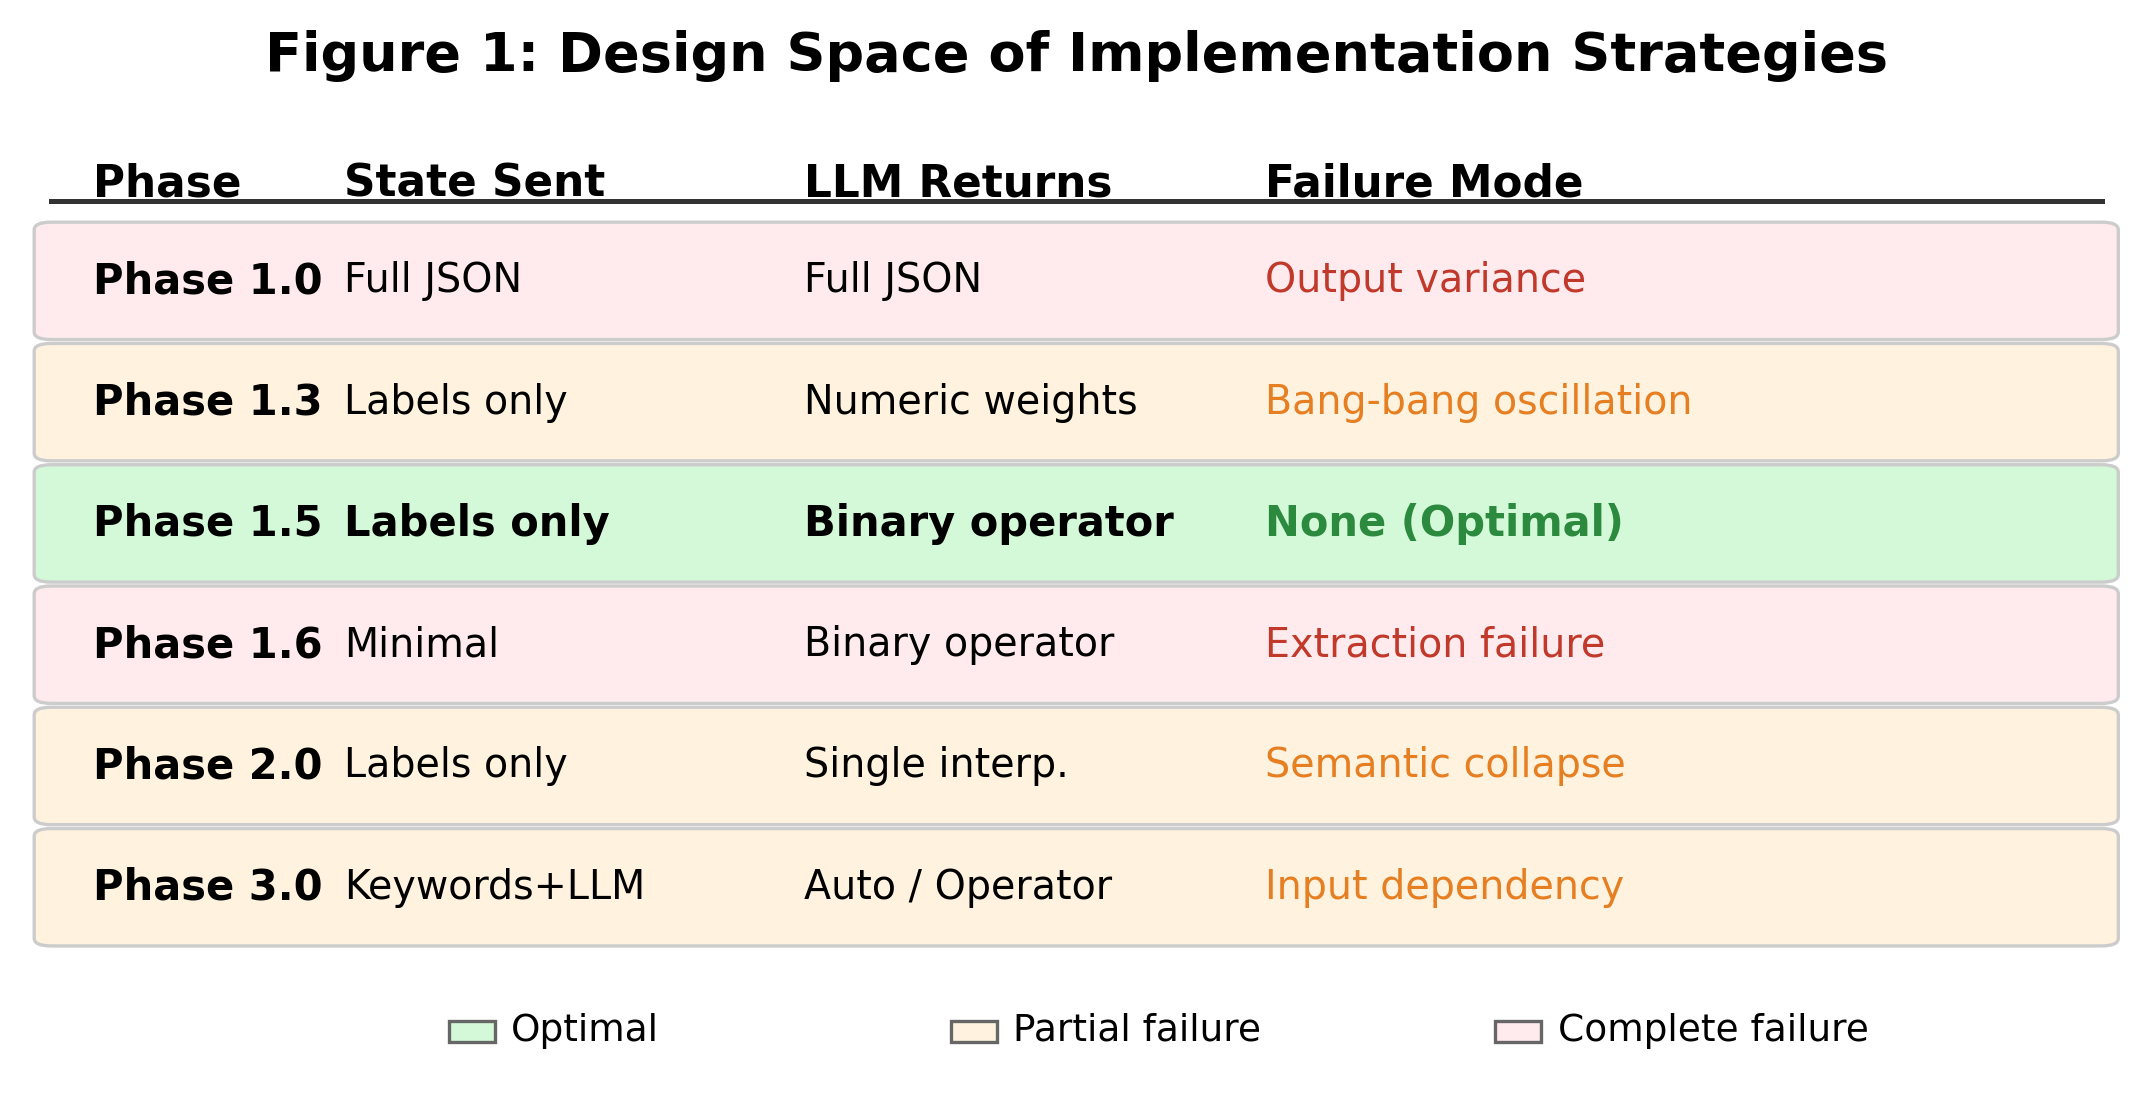
\includegraphics[width=0.95\textwidth]{fig1_design_space.png}
\caption{Design space of tested interface strategies. Green = only tested interface with no observed failure under this protocol, orange = partial failure (severity varies: Phase~1.3 produces valid output format but unstable weights; Phase~2.0 destroys multi-interpretation state entirely), red = complete failure.}
\label{fig:design_space}
\end{figure}

%==============================================================================
% SECTION 3: EXPERIMENTAL DESIGN
%==============================================================================
\section{Experimental Design}
\label{sec:design}

\subsection{Design Space}

We systematically vary two dimensions: (1)~what state information is sent to the LLM,
and (2)~what the LLM is asked to return. Table~\ref{tab:design_space} maps the six
strategies explored.

\begin{table}[ht]
\centering
\begin{tabular}{llll}
\toprule
\textbf{Phase} & \textbf{State Sent} & \textbf{LLM Returns} & \textbf{Tests} \\
\midrule
1.0 & Full JSON & Full JSON & Baseline \\
1.3 & Labels only & Numeric weights & Numeric precision \\
1.5 & Labels only & Binary operator & \textbf{No observed failure} \\
1.6 & Minimal & Binary operator & Prompt compression \\
2.0 & Labels only & Single interpretation & Semantic routing \\
3.0 & Keywords $\to$ auto / LLM & Hybrid & Input dependency \\
\bottomrule
\end{tabular}
\caption{Design space of implementation strategies}
\label{tab:design_space}
\end{table}

\subsection{Test Scenarios}

Three scenarios provide graduated complexity:

\textbf{Bank (5 turns, 2 interpretations):}
Financial institution vs.\ riverbank. Initial state:
\texttt{\{financial: 0.5, river: 0.5\}}. Inputs alternate between financial cues
(``Their interest rates just dropped'') and river cues (``Perfect for ducks and herons'').

\textbf{Spring (10 turns, 4 interpretations):}
Season vs.\ water source vs.\ mechanical coil vs.\ leap. Initial state:
\texttt{\{season: 0.4, water: 0.3, mechanical: 0.2, leap: 0.1\}}. Ten inputs
span all four interpretations.

\textbf{Court (12 turns, 4 interpretations):}
Legal vs.\ sports vs.\ royal court vs.\ courtship. Initial state:
\texttt{\{law: 0.35, sports: 0.30, royal: 0.25, romance: 0.10\}}. Twelve inputs
testing stability over extended conversations.

For Phase~3.0, each scenario has an additional \textbf{ambiguous} variant with
5 turns designed to contain zero keyword matches, forcing 100\% LLM fallback.

\subsection{Models}

All experiments use three commercial LLM APIs:
\begin{itemize}
    \item Claude Sonnet~4 (\texttt{claude-sonnet-4-20250514})
    \item GPT-4o-mini (\texttt{gpt-4o-mini-2024-07-18})
    \item Gemini~2.0~Flash (\texttt{gemini-2.0-flash})
\end{itemize}

\subsection{Parameters and Replication}

\begin{itemize}
    \item Temperature: 0.3 (realistic operating conditions)
    \item Max output tokens: 200
    \item Step size $\alpha$: 0.4
    \item Trials per experiment: 3
    \item Total runs: 45 experiments $\times$ 3 trials = 135
\end{itemize}

All experiments were executed on Google Colab under consistent API conditions
(123 runs in one session; 12 supplementary Phase~1.0 runs in a follow-up session).

\subsection{Evaluation Metrics}

\begin{itemize}
    \item \textbf{Token consumption}: Total and per-turn, reported as mean $\pm$ std
    across 3 trials
    \item \textbf{Extraction rate}: Percentage of turns where the expected output
    format was successfully parsed
    \item \textbf{Output variance}: Standard deviation of total tokens across trials
    (measures structural stability)
    \item \textbf{Weight volatility}: Mean absolute change in interpretation weights
    between consecutive turns (Phase~1.3 specific)
    \item \textbf{Semantic collapse rate}: Percentage of turns returning a single
    interpretation rather than preserving multiple (Phase~2.0 specific)
    \item \textbf{Commit-inertia proxies}: Reverse-action violations (captured in
    UCR complement) and OTAR/UCR drift persistence across sessions in the v55 extension
    \item \textbf{Automation rate}: Percentage of turns resolved by keyword matching
    without LLM calls (Phase~3.0 specific)
\end{itemize}

\noindent All standard deviations are reported as population standard deviations
(dividing by $N$, not $N{-}1$) since our 3 trials per configuration represent
the complete experimental population, not a sample from a larger one.
Cross-session variability (different API versions, load conditions) is
explicitly not modeled.

%==============================================================================
% SECTION 4: PHASE 1.0
%==============================================================================
\section{Phase 1.0: Naive Baseline}
\label{sec:phase1_0}

\subsection{Approach}

The most straightforward implementation: send the full NRR state as JSON, ask the
LLM to update weights, and return the complete updated state as JSON.

\begin{lstlisting}
prompt = f"""
Current NRR state (JSON):
{json.dumps(state, indent=2)}

New input: "{text}"
Update interpretation weights.
Return complete updated state as JSON.
"""
\end{lstlisting}

\subsection{Results}

\begin{table}[ht]
\centering
\begin{tabular}{llrrr}
\toprule
\textbf{Model} & \textbf{Scenario} & \textbf{Total tokens} & \textbf{Avg/turn} & \textbf{Std} \\
\midrule
Claude Sonnet 4 & Bank (5 turns) & 734 & 146.8 & $\pm$28.6 \\
                & Spring (10 turns) & 1979 & 197.9 & $\pm$47.7 \\
                & Court (12 turns) & 2498 & 208.2 & $\pm$17.4 \\
\midrule
GPT-4o-mini     & Bank (5 turns) & 877 & 175.3 & $\pm$58.4 \\
                & Spring (10 turns) & 2568 & 256.8 & $\pm$6.7 \\
                & Court (12 turns) & 2942 & 245.1 & $\pm$45.9 \\
\midrule
Gemini 2.0 Flash & Bank (5 turns) & 504 & 100.8 & $\pm$0.0 \\
                  & Spring (10 turns) & 1578 & 157.8 & $\pm$48.5 \\
                  & Court (12 turns) & 1871 & 155.9 & $\pm$2.4 \\
\bottomrule
\end{tabular}
\caption{Phase 1.0 performance across all model-scenario combinations (mean across 3 trials).
Total tokens grow linearly with turn count, confirming per-turn overhead is the dominant cost factor.}
\label{tab:phase1_0}
\end{table}

\subsection{Analysis}

Three problems are immediately apparent:

\textbf{High variance across models.} For the Bank scenario, total tokens range from 504 (Gemini) to
877 (GPT)---a 1.74$\times$ spread for identical inputs. This pattern persists across scenarios:
GPT consistently produces the most tokens (256.8 tokens/turn for Spring vs.\ Gemini's 157.8).
The LLM's verbosity in JSON reconstruction is unpredictable and model-dependent.

\textbf{High variance across trials.} GPT shows $\pm$58.4 standard deviation for Bank
and $\pm$45.9 for Court across just 3 trials. Gemini's Spring std reaches $\pm$48.5.
The ``return full JSON'' instruction gives the LLM too much output freedom, allowing
explanatory text, formatting variations, and verbose key names.

\textbf{Redundant transmission.} The full state is sent \textit{and} returned
every turn, even when only one interpretation weight changes. Per-turn cost scales
linearly with turn count across all scenarios, confirming that the full-state
round-trip is the dominant cost factor.

\textbf{Weight quality.} Preliminary inspection of Phase~1.0 weight trajectories
also reveals bang-bang oscillation similar to Phase~1.3 (§\ref{sec:phase1_3}),
suggesting the problem is intrinsic to LLM weight assignment rather than specific
to Phase~1.3's prompt format. This paper measures Phase~1.0 by token variance;
weight quality analysis across phases is deferred to future work.

%==============================================================================
% SECTION 5: PHASE 1.3
%==============================================================================
\section{Phase 1.3: Numeric Weight Return}
\label{sec:phase1_3}

\subsection{Hypothesis}

``If we send only interpretation labels (not full state) and ask the LLM to return
numeric weights, we reduce transmission overhead while maintaining precise control
over state evolution.''

This fills the gap between Phase~1.0 (send everything, return everything) and
Phase~1.5 (send labels, return binary operator). Phase~1.3 tests whether LLMs
can reliably assign \textit{precise numeric values} to interpretation weights.

\subsection{Implementation}

\begin{lstlisting}
prompt = f"""
Interpretations: [financial, river]

User input: "{text}"

Assign updated probability weights to each
interpretation. Weights must sum to 1.0.

Output ONLY in this format:
financial: <weight>
river: <weight>
"""
\end{lstlisting}

\subsection{Results}

\begin{table}[ht]
\centering
\begin{tabular}{lrrrr}
\toprule
\textbf{Model} & \textbf{Tokens} & \textbf{Parse rate} & \textbf{Volatility} & \textbf{Std} \\
\midrule
Claude & 448 & 100\% & 0.892 $\pm$ 0.006 & $\pm$0.0 \\
GPT & 383 & 100\% & 0.758 $\pm$ 0.024 & $\pm$0.5 \\
Gemini & 388 & 100\% & 0.900 $\pm$ 0.000 & $\pm$0.0 \\
\bottomrule
\end{tabular}
\caption{Phase 1.3 performance (Bank, 5 turns). Volatility = mean absolute weight
change between consecutive turns.}
\label{tab:phase1_3}
\end{table}

\subsection{The Bang-Bang Problem}

Parsing succeeds 100\% of the time---the LLM reliably outputs numbers that sum
to approximately 1.0. However, the \textit{content} of those numbers reveals a
fundamental problem. Table~\ref{tab:phase1_3_weights} shows weight trajectories
across turns.

\begin{table}[ht]
\centering
\begin{tabular}{clll}
\toprule
\textbf{Turn} & \textbf{Claude} & \textbf{GPT} & \textbf{Gemini} \\
\midrule
1 (ambig.) & 0.90 / 0.10 & 0.80 / 0.20 & 0.95 / 0.05 \\
2 (river) & 0.05 / 0.95 & 0.10 / 0.90 & 0.05 / 0.95 \\
3 (finan.) & 1.00 / 0.00 & 0.90 / 0.10 & 0.95 / 0.05 \\
4 (river) & 0.10 / 0.90 & 0.20 / 0.80 & 0.05 / 0.95 \\
5 (finan.) & 0.95 / 0.05 & 0.90 / 0.10 & 0.95 / 0.05 \\
\bottomrule
\end{tabular}
\caption{Phase 1.3 weight trajectories (financial / river). Values shown are
from trial~1; trials~2 and~3 are nearly identical.}
\label{tab:phase1_3_weights}
\end{table}

Every model exhibits \textbf{bang-bang behavior}: weights swing between near-zero
and near-one on each turn. The mean absolute weight change per turn (volatility)
is 0.76--0.90 across models, indicating near-total weight reversal each
turn rather than the gradual evolution Phase~1.5 achieves through client-side
normalization. Figure~\ref{fig:bangbang} visualizes these trajectories.

\begin{figure}[ht]
\centering
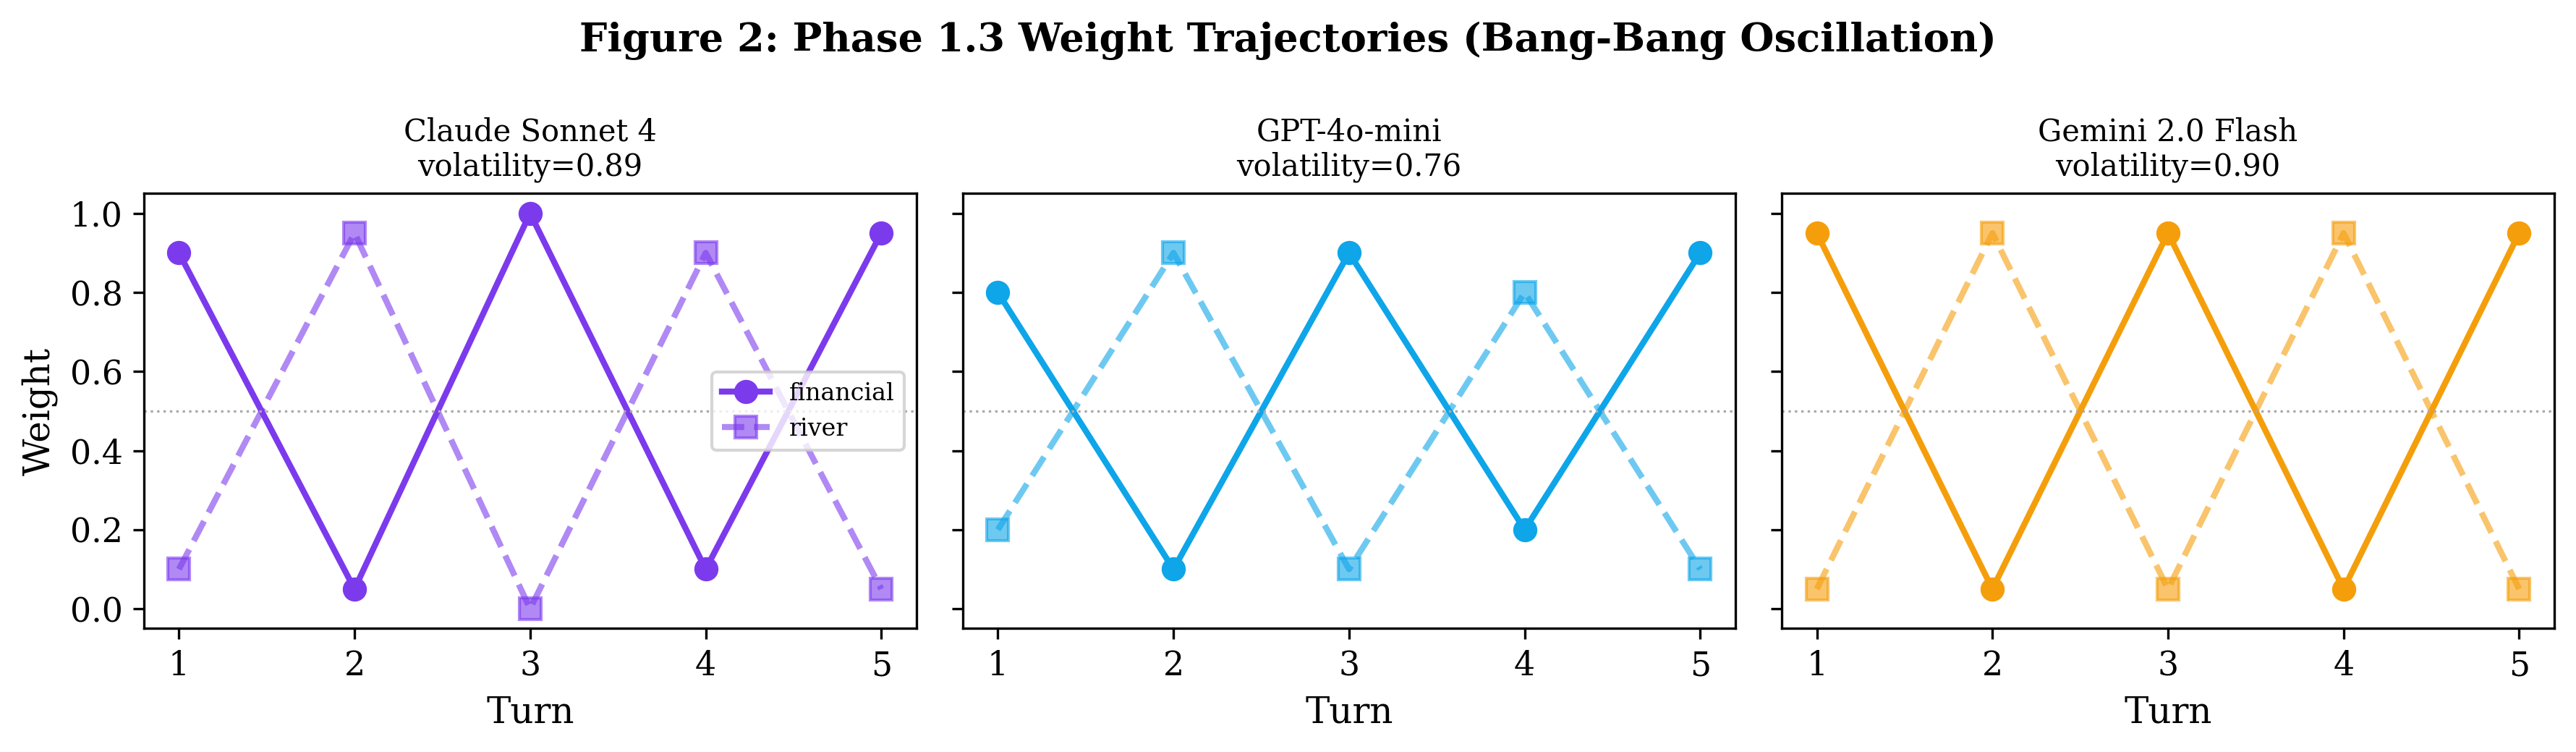
\includegraphics[width=\textwidth]{fig2_bangbang.png}
\caption{Phase 1.3 weight trajectories for the Bank scenario (trial~1).
All three models exhibit bang-bang oscillation between near-0 and near-1 weights.
Volatility values are 3-trial means, matching Table~\ref{tab:phase1_3}.}
\label{fig:bangbang}
\end{figure}

This occurs because the LLM treats each turn as an independent classification task:
``this input sounds financial, so financial $\approx$ 0.9.'' It does not perform
incremental updates---it reassigns from scratch. The result is that NRR's core
principle of \textit{gradual} meaning evolution is violated. When Turn~3 assigns
financial = 1.00 and river = 0.00, the river interpretation is effectively pruned,
destroying the ambiguity that NRR exists to preserve.

\textbf{Conclusion}: LLMs can produce well-formatted numeric outputs but cannot
perform controlled incremental state updates. Numeric precision is not the
bottleneck---\textit{update discipline} is.

%==============================================================================
% SECTION 6: PHASE 1.5
%==============================================================================
\section{Phase 1.5: Operator Abstraction}
\label{sec:phase1_5}

\subsection{Design Insight}

Phase~1.3 demonstrated that asking the LLM for \textit{numeric values} fails because
the LLM cannot maintain incremental update discipline. The solution: \textbf{don't
ask the LLM for numbers at all.} Instead, ask for a binary directional decision
($\sigma$ or $\delta$) and let the client handle all arithmetic.

Function calling and JSON mode constrain output format, but they do not constrain
output content. Phase~1.5 additionally constrains output content to a binary
action space (sigma/delta plus target), and the six-phase comparison
shows this avoids the Phase~1.0--1.3 failure pattern under the tested setup.

\subsection{Implementation}

\begin{lstlisting}
prompt = f"""
Current state: {state_id}
Interpretations: {list(state.keys())}

User input: "{text}"

Available operators:
- sigma (strengthen): Increase weight
- delta (dampen): Decrease weight

Output ONLY in this format:
operator: <sigma or delta>
target: <interpretation_key>
"""
\end{lstlisting}

The \texttt{state\_id} is an opaque reference token (e.g., \texttt{state\_bank\_001})
that the LLM receives but cannot interpret---it exists solely as a placeholder
to maintain prompt structure without transmitting actual state data. The client
maintains state externally. On receiving the LLM's response, it applies:
\begin{align}
\sigma(m_i) &: w_i \leftarrow \min(1.0,\; w_i + \alpha) \\
\delta(m_i) &: w_i \leftarrow \max(0.0,\; w_i - \alpha)
\end{align}
followed by renormalization: $w_i \leftarrow w_i / \sum_j w_j$.

\subsection{Cross-Model Results}

\begin{table}[ht]
\centering
\begin{tabular}{lrrrr}
\toprule
\textbf{Model} & \textbf{Bank (5t)} & \textbf{Spring (10t)} & \textbf{Court (12t)} & \textbf{Extract} \\
\midrule
Claude & 513 $\pm$ 0 & 1108 $\pm$ 0 & 1316 $\pm$ 0 & 100\% \\
GPT & 449 $\pm$ 0 & 987 $\pm$ 0 & 1181 $\pm$ 0 & 100\% \\
Gemini & 458 $\pm$ 0 & 978 $\pm$ 0 & 1179.3 $\pm$ 0.5 & 100\% \\
\bottomrule
\end{tabular}
\caption{Phase 1.5 total tokens across all scenarios (mean $\pm$ std, 3 trials).
Extraction rate is 100\% across all 9 model-scenario combinations (27 total runs).}
\label{tab:phase1_5}
\end{table}

\subsection{Structural Stability}

The most striking result: \textbf{standard deviation is near-zero across all trials.}
At temperature~0.3, Phase~1.5 produces identical or near-identical token counts in every
run (max observed std = 0.5 tokens for one configuration; all others are exactly zero).
The output is so tightly constrained (two words: an operator
and a target) that any variation fits within the same or adjacent token count.

This structural stability is unique to Phase~1.5. Phase~1.0 shows variance
up to $\pm$58.4 tokens (GPT, Bank), and Phase~1.6 shows $\pm$35.9--54.2.

\subsection{Cross-Scenario Stability}

Table~\ref{tab:phase1_5_avg} shows per-turn token consumption across scenarios.

\begin{table}[ht]
\centering
\begin{tabular}{lrrr}
\toprule
\textbf{Model} & \textbf{Bank (5t)} & \textbf{Spring (10t)} & \textbf{Court (12t)} \\
\midrule
Claude & 102.6 & 110.8 & 109.7 \\
GPT & 89.8 & 98.7 & 98.4 \\
Gemini & 91.6 & 97.8 & 98.3 \\
\bottomrule
\end{tabular}
\caption{Phase 1.5 average tokens per turn. All values have std $\leq$ 0.5 across trials.}
\label{tab:phase1_5_avg}
\end{table}

Figure~\ref{fig:stability} visualizes the narrow performance band across all
model-scenario combinations.

\begin{figure}[ht]
\centering
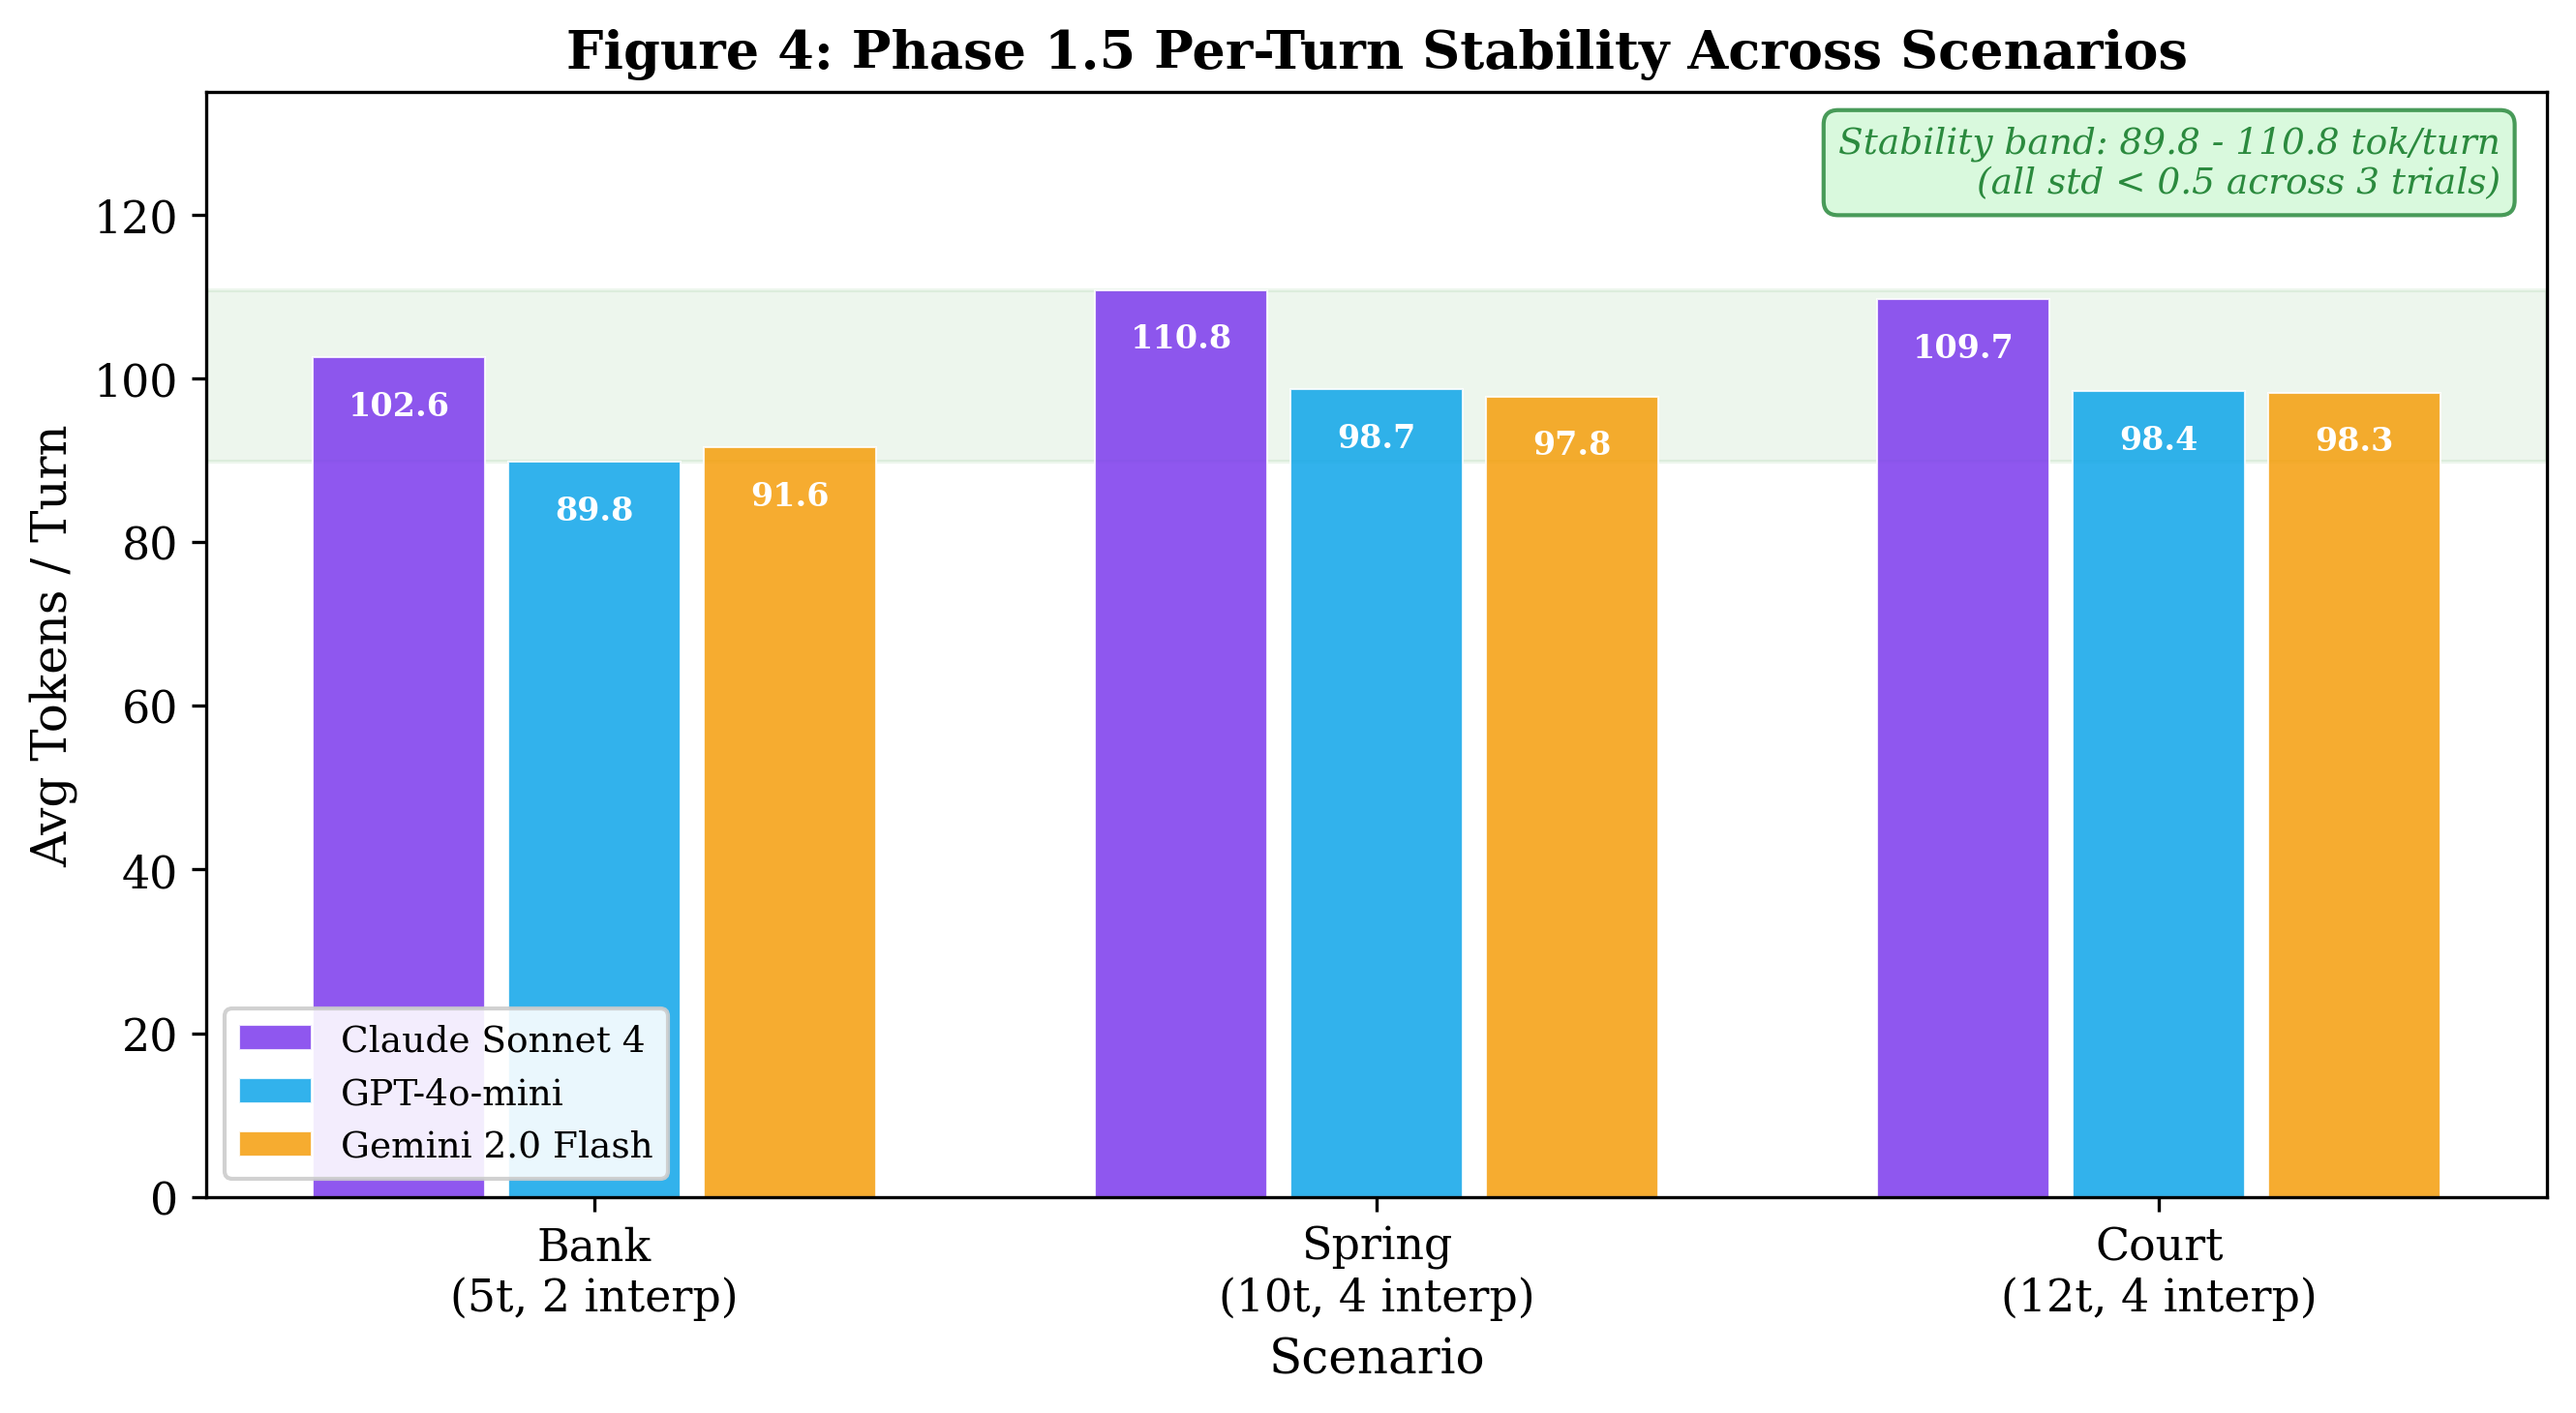
\includegraphics[width=0.85\textwidth]{fig4_stability.png}
\caption{Phase 1.5 per-turn token consumption across scenarios and models.
All 9 combinations fall within a 89.8--110.8 tokens/turn band (std $\leq$ 0.5).}
\label{fig:stability}
\end{figure}

Per-turn consumption falls in a narrow band of 89.8--110.8 tokens/turn across all
9 model-scenario combinations. Doubling the number of interpretations (Bank: 2
$\rightarrow$ Spring/Court: 4) increases per-turn cost by only 6.8--9.9\%,
demonstrating near-independence from state complexity.

\subsection{Operator Distribution}

\begin{table}[ht]
\centering
\begin{tabular}{llrr}
\toprule
\textbf{Scenario} & \textbf{Model} & \textbf{$\sigma$ (\%)} & \textbf{$\delta$ (\%)} \\
\midrule
\multirow{3}{*}{Bank} & Claude & 100 & 0 \\
 & GPT & 60 & 40 \\
 & Gemini & 100 & 0 \\
\midrule
\multirow{3}{*}{Spring} & Claude & 100 & 0 \\
 & GPT & 83 & 17 \\
 & Gemini & 90 & 10 \\
\midrule
\multirow{3}{*}{Court} & Claude & 100 & 0 \\
 & GPT & 94 & 6 \\
 & Gemini & 100 & 0 \\
\bottomrule
\end{tabular}
\caption{Phase 1.5 operator distribution (mean across 3 trials, rounded to nearest integer).
Claude is $\sigma$-only; Gemini is mostly $\sigma$ with limited $\delta$ in Spring;
GPT shows scenario-dependent $\delta$ usage.}
\label{tab:phase1_5_ops}
\end{table}

Claude consistently chooses $\sigma$ (strengthen the matching
interpretation). Gemini is also $\sigma$-dominant (with limited $\delta$ in Spring),
while GPT occasionally uses $\delta$ (dampen an alternative).
Both strategies are valid---they produce different weight trajectories but
converge to the same relative ordering. The key observation is that all models
reliably select a valid operator-target pair regardless of their strategic
preference, confirming that the binary decision space is within all models'
reliable capabilities.

%==============================================================================
% SECTION 7: PHASE 1.6
%==============================================================================
\section{Phase 1.6: Over-Compressed Prompts}
\label{sec:phase1_6}

\subsection{Hypothesis}

``If reducing prompt verbosity helped (Phase~1.0 $\rightarrow$ 1.5), reducing it
further should help more.''

\subsection{Implementation}

\begin{lstlisting}
prompt = f"""
{list(state.keys())}
"{text}"
op? tgt?
"""
\end{lstlisting}

This strips all instructional context: no operator definitions, no format
specification, no state identifier.

\subsection{Results}

\begin{table}[ht]
\centering
\begin{tabular}{lrrr}
\toprule
\textbf{Model} & \textbf{Tokens (mean)} & \textbf{Std} & \textbf{Extraction rate} \\
\midrule
Claude & 707 & $\pm$54.2 & 0\% \\
GPT & 772 & $\pm$49.2 & 0\% \\
Gemini & 404 & $\pm$35.9 & 0\% \\
\bottomrule
\end{tabular}
\caption{Phase 1.6 performance (Bank, 5 turns). Extraction rate is 0\% for
all models across all 9 runs.}
\label{tab:phase1_6}
\end{table}

\subsection{Analysis: Universal Failure}

Unlike Phase~1.3 (which parses correctly but oscillates) or Phase~2.0
(which is cheap but collapses), Phase~1.6 fails at the most basic level:
\textbf{no model can produce the expected output format.}

Without explicit operator definitions and format instructions, all three models
generate free-form responses: explanations, questions, multi-sentence analyses.
None produce the ``operator: X / target: Y'' format required for automated
extraction.

Furthermore, output variance is high ($\pm$35.9--54.2), confirming that
unconstrained output leads to unpredictable token consumption---the same problem
as Phase~1.0 but worse, because the outputs are not even parseable.

\textbf{Conclusion}: There exists a minimum instruction threshold below which
LLMs cannot perform structured tasks. Phase~1.5's prompt is not merely
``shorter than 1.0''---it is precisely calibrated to provide sufficient context
for reliable extraction while minimizing overhead.

%==============================================================================
% SECTION 8: PHASE 2.0
%==============================================================================
\section{Phase 2.0: Classification-Based Routing}
\label{sec:phase2_0}

\subsection{Hypothesis}

``Use single-interpretation classification instead of operator selection. Ask the LLM
which interpretation best matches the input, then route accordingly.''

\subsection{Implementation}

Turn~1 generates semantic descriptions for each interpretation via LLM.
Subsequent turns ask the LLM: ``Which interpretation is most similar to
this input?'' and expect a single interpretation name in response. Note that
despite the conceptual framing as ``similarity matching,'' no actual embedding
vectors are computed; the LLM performs classification in natural language.

\subsection{Results}

\begin{table}[ht]
\centering
\begin{tabular}{lrrr}
\toprule
\textbf{Model} & \textbf{Tokens (mean)} & \textbf{Std} & \textbf{Collapse rate} \\
\midrule
Claude & 429 & $\pm$0 & 100\% \\
GPT & 368 & $\pm$15.7 & 100\% \\
Gemini & 367 & $\pm$0 & 100\% \\
\bottomrule
\end{tabular}
\caption{Phase 2.0 performance (Bank, 5 turns). Collapse rate = percentage of
classification turns (turns 2--5) returning a single interpretation; turn~1 is a
setup turn generating semantic descriptions.}
\label{tab:phase2_0}
\end{table}

\subsection{Semantic Collapse}

Phase~2.0 is token-efficient---cheaper than Phase~1.5 for all models. If token
cost were the only metric, it would appear superior. But examining the outputs
reveals the fatal flaw:

\begin{quote}
Turn 2: ``river'' \\
Turn 3: ``financial'' \\
Turn 4: ``river'' \\
Turn 5: ``financial''
\end{quote}

Every model, on every trial, returns \textbf{exactly one interpretation per turn}.
The response alternates between ``river'' and ``financial'' as a binary
classification, with no mechanism for expressing that both interpretations remain
plausible.

This is semantic collapse: the NRR state degenerates from a weighted distribution
$\{$financial: 0.65, river: 0.35$\}$ to a point estimate $\{$financial: 1.0$\}$.
The core principle of non-resolution---maintaining multiple interpretations
simultaneously---is destroyed.

\textbf{Conclusion}: Asking ``which interpretation matches?'' forces the LLM into
classification mode. Classification is inherently resolution-based: it must pick
one answer. NRR requires a fundamentally different output structure---one that
preserves ambiguity. Phase~1.5's operator abstraction achieves this by asking
\textit{which interpretation to adjust}, not \textit{which interpretation is
correct}.

%==============================================================================
% SECTION 9: PHASE 3.0
%==============================================================================
\section{Phase 3.0: Hybrid Router}
\label{sec:phase3_0}

\subsection{Hypothesis}

``For domain-specific applications, keyword matching can resolve many turns
without any LLM call. Use LLM only as fallback for ambiguous inputs.''

\subsection{Implementation}

Each scenario has a pre-defined keyword dictionary mapping keywords to
interpretations. On each turn:
\begin{enumerate}
    \item Check if the input contains any keyword from the dictionary.
    \item If a match is found: apply $\sigma$ to the matched interpretation
    automatically (zero tokens).
    \item If no match: fall back to Phase~1.5's LLM-based operator selection.
\end{enumerate}

\subsection{Results: Explicit Inputs}

\begin{table}[ht]
\centering
\begin{tabular}{lrrrr}
\toprule
\textbf{Scenario} & \textbf{Auto rate} & \textbf{Claude} & \textbf{GPT} & \textbf{Gemini} \\
\midrule
Bank & 80\% & 20.4/t & 18.0/t & 18.4/t \\
Spring & 90\% & 11.2/t & 10.1/t & 10.0/t \\
Court & 100\% & 0.0/t & 0.0/t & 0.0/t \\
\bottomrule
\end{tabular}
\caption{Phase 3.0 with explicit inputs (avg tokens/turn). All values have
std = 0 across 3 trials.}
\label{tab:phase3_0_explicit}
\end{table}

With keyword-rich inputs, Phase~3.0 achieves dramatic efficiency. The Court
scenario achieves \textbf{100\% automation with zero LLM calls}: every turn
contains an unambiguous keyword.

\subsection{Results: Ambiguous Inputs}

\begin{table}[ht]
\centering
\begin{tabular}{lrrrr}
\toprule
\textbf{Scenario} & \textbf{Auto rate} & \textbf{Claude} & \textbf{GPT} & \textbf{Gemini} \\
\midrule
Bank & 0\% & 105.0/t & 92.8/t & 95.2/t \\
Spring & 0\% & 114.2/t & 102.6/t & 101.6/t \\
Court & 0\% & 112.6/t & 101.6/t & 101.6/t \\
\bottomrule
\end{tabular}
\caption{Phase 3.0 with ambiguous inputs (avg tokens/turn). All values have
std = 0 across 3 trials.}
\label{tab:phase3_0_ambiguous}
\end{table}

With ambiguous inputs (designed to contain zero keywords), automation drops to
\textbf{0\% across all scenarios and models}. Every turn falls back to the LLM,
and per-turn costs reach 92.8--114.2 tokens/turn, comparable to Phase~1.5
(89.8--110.8).

\subsection{The Input Dependency Problem}

Phase~3.0's performance is entirely determined by input characteristics, not by
the system's own capabilities:

\begin{itemize}
    \item Explicit inputs: 80--100\% automation, near-zero cost
    \item Ambiguous inputs: 0\% automation, full Phase~1.5 cost
\end{itemize}

This binary behavior means Phase~3.0 cannot serve as a general-purpose strategy.
It excels in narrow, well-defined domains (e.g., customer support with standard
terminology) but provides no benefit when inputs are naturally ambiguous---precisely
the case where NRR is most needed.

\textbf{Conclusion}: Keyword-based routing is a valid optimization for known
domains but cannot replace general-purpose operator abstraction. Phase~1.5
handles both explicit and ambiguous inputs with consistent performance.

%==============================================================================
% SECTION 10: COMPARATIVE ANALYSIS
%==============================================================================
\section{Comparative Analysis}
\label{sec:comparative}

\subsection{Summary Table}

\begin{table}[ht]
\centering
\small
\begin{tabular}{lrrllll}
\toprule
\textbf{Phase} & \textbf{Tokens} & \textbf{Std} & \textbf{Extract} & \textbf{NRR OK?} & \textbf{Failure mode} \\
\midrule
1.0 & 734 & $\pm$29 & --- & Partial$^\dagger$ & Output variance \\
1.3 & 448 & $\pm$0 & 100\% & \textbf{No} & Bang-bang oscillation \\
\textbf{1.5} & \textbf{513} & $\leq$\textbf{0.5} & \textbf{100\%} & \textbf{Yes} & \textbf{None} \\
1.6 & 707 & $\pm$54 & 0\% & No & Universal extraction failure \\
2.0 & 429 & $\pm$0 & --- & \textbf{No} & Semantic collapse \\
3.0e & 102 & $\pm$0 & 80\%$^*$ & Cond.$^\ddagger$ & Input dependency \\
3.0a & 525 & $\pm$0 & 0\%$^*$ & Yes & (reverts to 1.5) \\
\bottomrule
\end{tabular}
\caption{Comparative summary (Bank scenario, Claude, mean across 3 trials).
$^*$Phase 3.0 extraction refers to automation rate, not operator extraction.
$^\dagger$Phase 1.0 returns full JSON including weights, so multiple
interpretations are nominally preserved; however, weight quality is not analyzed
in this paper (only token variance is measured).
$^\ddagger$Phase 3.0 explicit preserves NRR for keyword-matched inputs but
provides no guarantee for ambiguous inputs, where it falls back to Phase~1.5.}
\label{tab:comparative}
\end{table}

Figure~\ref{fig:comparative} visualizes the token consumption and variance
across all phases.

\begin{figure}[ht]
\centering
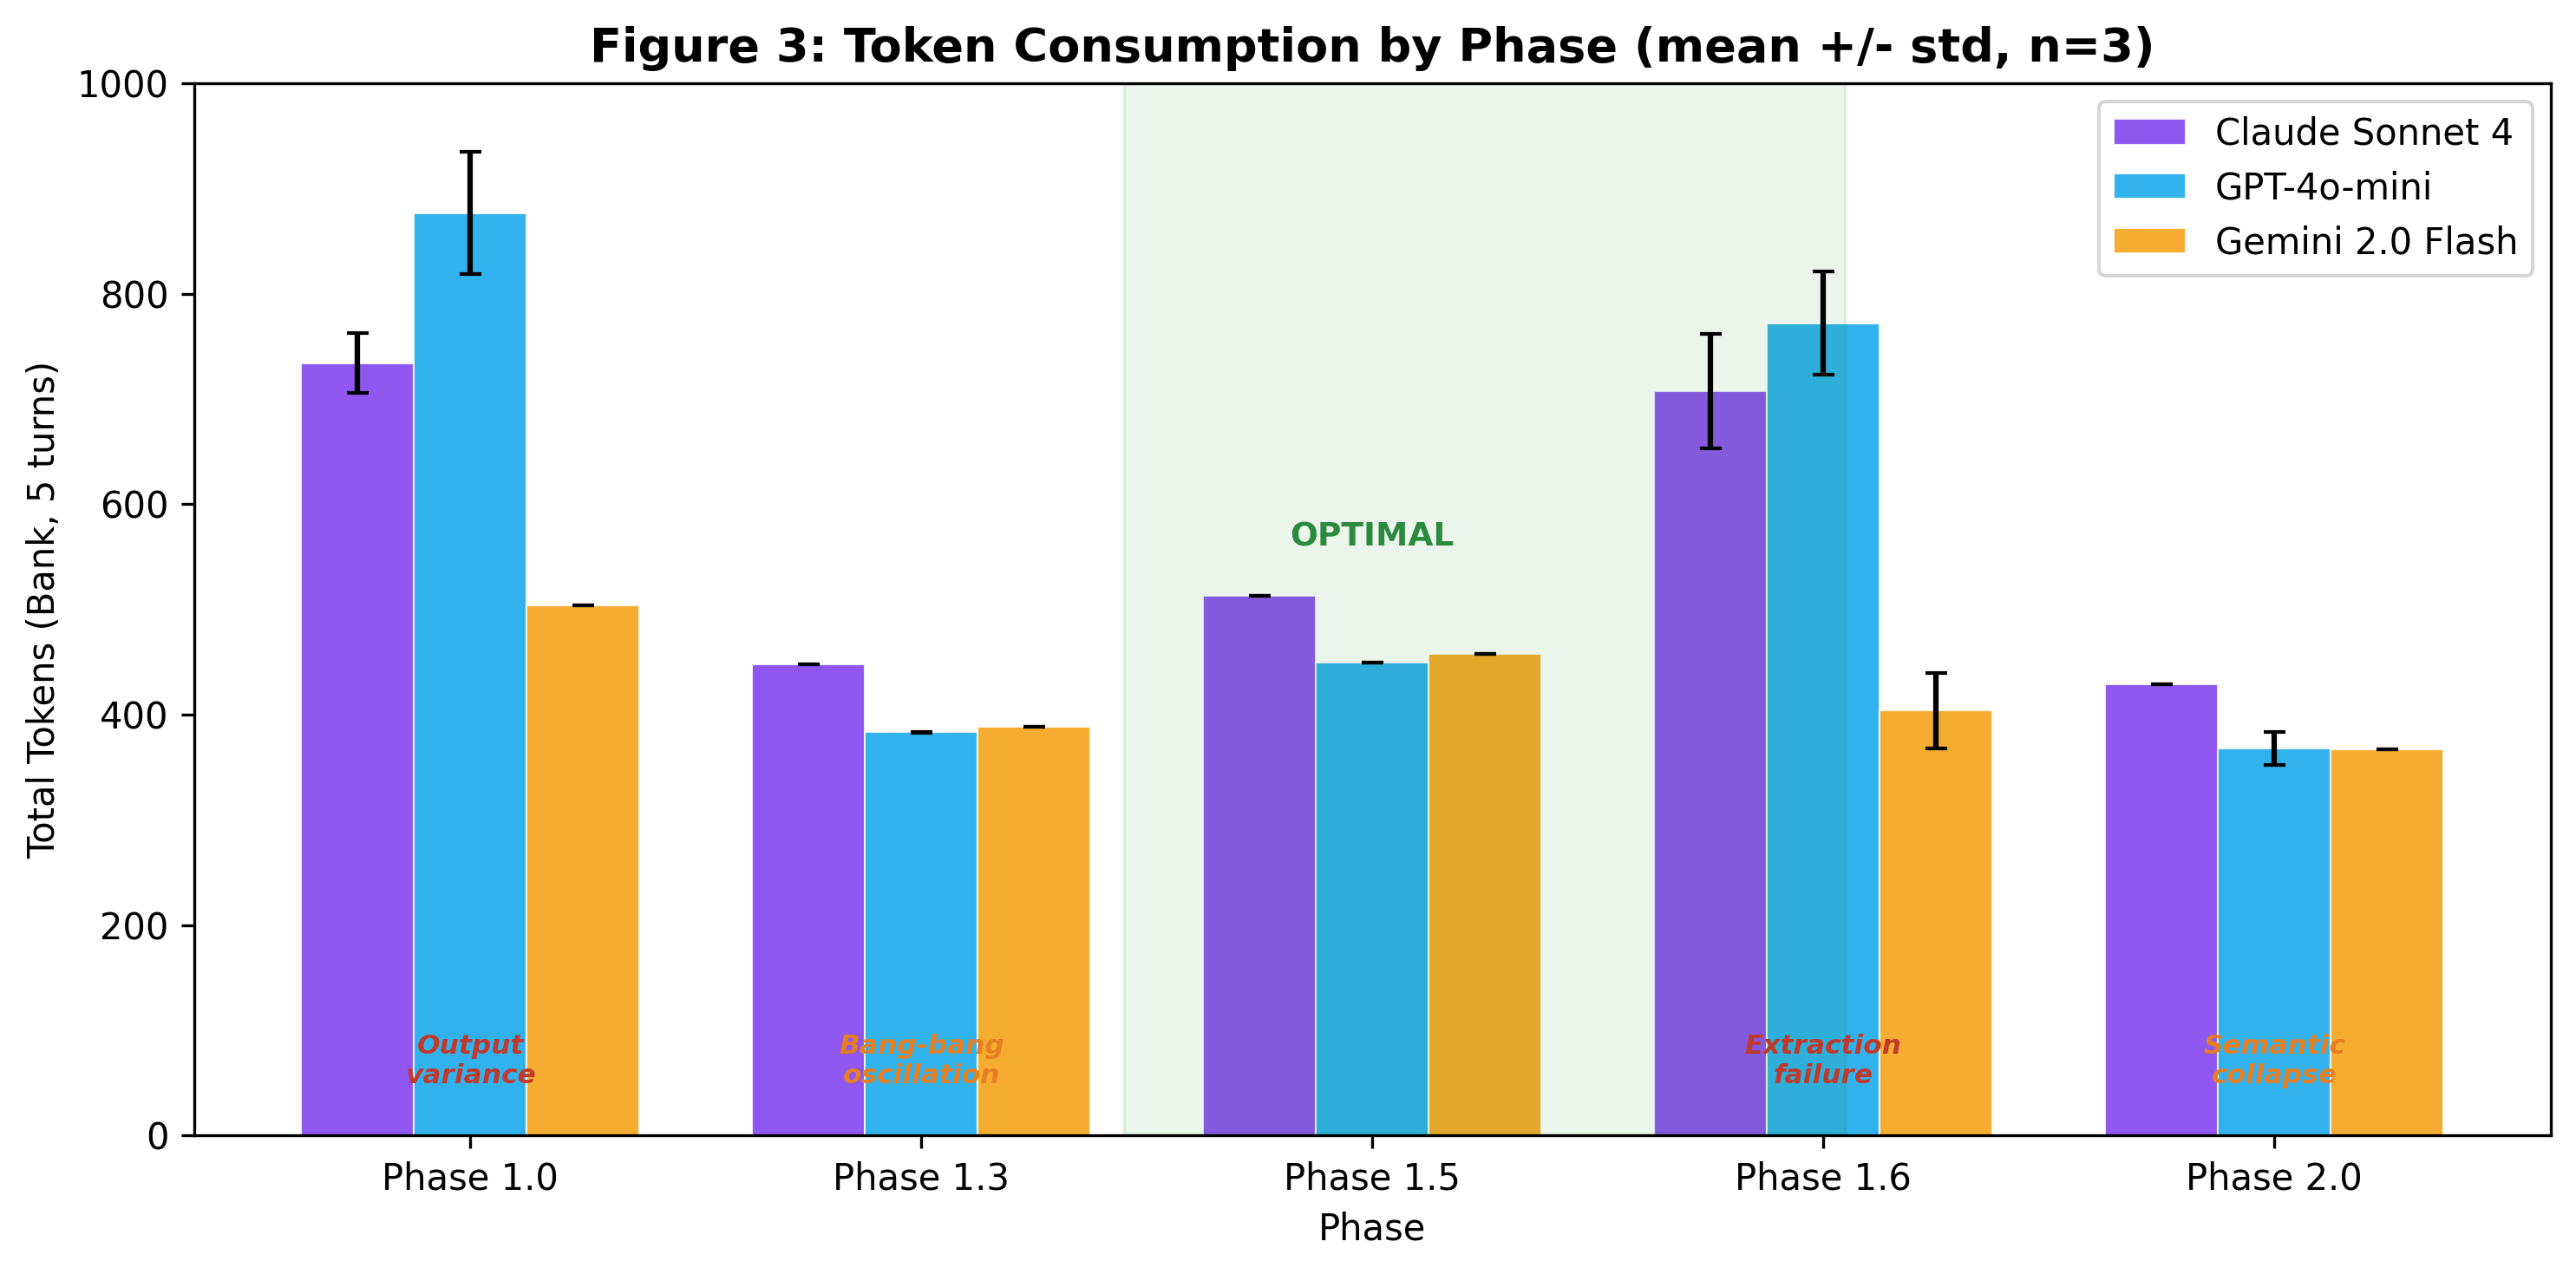
\includegraphics[width=0.95\textwidth]{fig3_comparative.png}
\caption{Token consumption by phase (Bank scenario, mean $\pm$ std across 3 trials).
Phase~1.5 combines low cost with near-zero variance. Failure mode annotations
indicate the primary limitation of each alternative strategy. Phase~3.0 is omitted
because its token consumption is input-dependent (0 for keyword-matched, Phase~1.5-equivalent for ambiguous).}
\label{fig:comparative}
\end{figure}

\subsection{Failure Taxonomy}

The four failure modes occupy distinct dimensions, confirming that Phase~1.5's
success is not merely ``avoiding one problem'' but satisfying multiple orthogonal
requirements simultaneously:

\begin{enumerate}
    \item \textbf{Output variance / Extraction failure} (Phase 1.0, 1.6):
    Unconstrained output format leads to unpredictable token consumption
    (Phase~1.0) and complete extraction failure (Phase~1.6, 0\% success).
    Both stem from allowing the LLM to determine its own output structure,
    but manifest differently: Phase~1.0 returns parseable JSON with high
    variance, while Phase~1.6 embeds answers in free-form text that resists
    automated extraction.

    \item \textbf{Weight oscillation} (Phase 1.3): The LLM produces well-formatted
    output but cannot maintain incremental update discipline. Each turn is treated
    as independent classification, violating NRR's gradual evolution principle.

    \item \textbf{Semantic collapse} (Phase 2.0): The LLM is forced into
    single-answer classification, destroying the multi-interpretation state
    that NRR exists to preserve. Token efficiency is high but meaningless---the
    system is no longer performing NRR.

    \item \textbf{Input dependency} (Phase 3.0): Performance varies from optimal
    to baseline depending entirely on input characteristics, providing no
    guaranteed efficiency for general-purpose deployment.
\end{enumerate}

\subsection{Why Phase 1.5 Succeeds}

Phase~1.5 avoids all four failure modes through a single design decision:
\textbf{constrain the LLM to binary directional decisions and delegate all
numeric computation to the client.}

This separation of concerns works because:
\begin{itemize}
    \item Binary decisions ($\sigma/\delta$ + target) are within all LLMs'
    reliable capabilities $\rightarrow$ 100\% extraction rate
    \item The output space is so constrained that temperature has no effect
    $\rightarrow$ near-zero variance
    \item Numeric state evolution is handled by deterministic client code
    $\rightarrow$ no oscillation, no collapse
    \item No dependence on input keywords $\rightarrow$ consistent performance
    regardless of input characteristics
\end{itemize}

%==============================================================================
% SECTION 11: DISCUSSION
%==============================================================================
\section{Discussion}
\label{sec:discussion}

\subsection{Generalizable Principles}

The findings extend beyond IME to any stateful reasoning system on stateless APIs:

\begin{principle}[Minimum Output Constraint]
LLM outputs must be constrained to the minimum decision space required. ``Return
a number'' is less reliable than ``return a direction.'' The narrower the output
space, the higher the structural stability.
\end{principle}

\begin{principle}[Client-Side Computation]
All deterministic computation (arithmetic, normalization, state updates) should
be performed by client code, not by the LLM. LLMs should make qualitative
judgments; clients should execute quantitative operations.
\end{principle}

\begin{principle}[Interface Constraint as Stability Mechanism]
Interface constraints serve not just as parsing aids but as stability
mechanisms. Phase~1.5's near-zero variance is a direct consequence of its
return-structure constraint, not of temperature settings.
\end{principle}

\begin{principle}[Non-Resolution Requires Non-Classification]
Any output format that forces the LLM to choose ``the best'' interpretation
will produce semantic collapse. Preserving ambiguity requires output structures
that reference interpretations without resolving them.
\end{principle}

\subsection{Collapse vs Commit Inertia}

We distinguish two different failure targets. Collapse is a point event:
the system selects a concrete output at a turn. Commit inertia is a trajectory
effect: after selection, future updates remain overly anchored to prior choices
despite new evidence. IME's practical objective is therefore not ``no collapse'',
but low premature-commit inertia under explicit conditions, with reversible
update paths maintained by client-side deterministic state control.

\subsection{The Structural Stability Phenomenon}

Phase~1.5's near-zero variance across trials at temperature~0.3 warrants further
discussion. This is not a trivial result---it means that \textbf{interface
design alone can create near-deterministic behavior from a stochastic system.}

The mechanism is output space compression: when the valid output is approximately
``operator: sigma / target: financial'' (roughly 10 tokens), the probability
distribution over possible completions is so peaked that temperature~0.3
introduces negligible variation (max observed std = 0.5 tokens across all
configurations). This contrasts with Phase~1.0, where the
output space (full JSON with explanations) is large enough for temperature to
produce meaningful variation ($\pm$28--58 tokens).

This suggests a design heuristic: if you need reproducible behavior from
stochastic APIs, \textbf{shrink the decision interface rather than merely
lowering the temperature.} Lowering temperature alone does not reduce output
space size; Phase~1.5 achieves stability through structural constraint on what
can be generated, not through sampling suppression.

\subsection{Cross-Model Consistency}

All three models achieve 100\% extraction on Phase~1.5 despite representing
different architectures, training data, and instruction-following capabilities.
This suggests that binary operator selection is below the ``reliability floor''
for current LLMs---a task so simple that model differences become irrelevant.

The operator \textit{strategy} differs across models (Claude uses 100\%
$\sigma$; GPT uses a mix of $\sigma$ and $\delta$), but this is a feature,
not a bug: both strategies produce valid state updates within the NRR framework.

\subsection{Supplementary v55 Re-Experiment (Post-v54 Reinforcement)}

To reduce four review risks (alpha fixed-point dependency, limited scale,
cross-session robustness, and interface-success vs.\ update-quality gap), we
ran a supplementary v55 protocol after the main 135-run comparison.

\textbf{Protocol scope.}
\begin{itemize}
    \item E1 (alpha sensitivity): 270 runs
    \item E2 (scale stress): 45 runs
    \item E3 (cross-session): 108 runs in four sessions (\texttt{a,b,c,d})
\end{itemize}
Total analyzed valid runs: 423 (5{,}562 turns). Infrastructure-failure logs
from earlier setup attempts were excluded by explicit file selection.

\textbf{Aggregate outcomes (v55 extension).}
\begin{itemize}
    \item ESR: 0.9975 overall (E1: 1.000, E2: 0.9935, E3: 1.000)
    \item OTAR/UCR: 0.8326 / 0.8351 overall
    \item Session-drift (aggregate): relative to session~a, sessions~b and~d
    remained within pre-registered bounds, while session~c exceeded the OTAR/UCR
    drift bound ($|\Delta|=0.0412 > 0.03$) despite token drift staying small
    ($\Delta$ tokens/turn $=0.033$).
\end{itemize}

\begin{table}[ht]
\centering
\begin{tabular}{lrrrr}
\toprule
\textbf{Mode} & \textbf{Turns} & \textbf{ESR} & \textbf{OTAR} & \textbf{UCR} \\
\midrule
E1 & 2430 & 1.000 & 0.849 & 0.849 \\
E2 & 2160 & 0.994 & 0.815 & 0.822 \\
E3 & 972 & 1.000 & 0.831 & 0.831 \\
\midrule
Overall & 5562 & 0.997 & 0.833 & 0.835 \\
\bottomrule
\end{tabular}
\caption{Supplementary v55 aggregate quality-proxy metrics (valid-only analysis set).}
\label{tab:v55_mode_metrics}
\end{table}

\begin{table}[ht]
\centering
\begin{tabular}{lrrr}
\toprule
\textbf{Session} & $\Delta$ tokens/turn & $|\Delta\text{OTAR}|$ & $|\Delta\text{UCR}|$ \\
\midrule
b (vs.\ a) & 0.041 & 0.004 & 0.004 \\
c (vs.\ a) & 0.033 & 0.041 & 0.041 \\
d (vs.\ a) & -0.218 & 0.021 & 0.021 \\
\bottomrule
\end{tabular}
\caption{Session-drift aggregate comparison in v55 extension (reference=session~a).
Pre-registered bounds: $|\Delta\text{tokens/turn}| \le 2.0$, $|\Delta\text{OTAR}| \le 0.03$, $|\Delta\text{UCR}| \le 0.03$.}
\label{tab:v55_session_drift}
\end{table}

\textbf{Condition-level boundary behavior.}
At model$\times$scenario resolution, 10/27 session comparisons exceeded at least
one drift threshold, concentrated in:
\begin{itemize}
    \item Claude--Bank (3 cases),
    \item GPT--Spring (3 cases),
    \item Claude--Court (2 cases),
    \item Claude--Spring (2 cases).
\end{itemize}

These results support a conditional interpretation: under tested settings,
Phase~1.5 remains operationally stable at aggregate level, but non-effective
regions persist in specific model-scenario conditions and must be reported
explicitly rather than averaged away.

\subsection{Limitations}

\textbf{Scenario scope.} All experimental inputs are in English with clear semantic
boundaries. Cross-lingual robustness is untested. Performance on highly
ambiguous or domain-specific inputs requires further study.
Phases~1.3, 1.6, and~2.0 were tested on the Bank scenario only; their failure
modes may manifest differently in multi-interpretation scenarios (Spring, Court).

\textbf{Operator set.} This paper tests only $\sigma$ and $\delta$. The full
NRR operator set ($\tau$, $\kappa$, $\pi$; defined in \cite{saito2026phi}, Appendix~D) may require richer output formats,
potentially reducing the structural stability advantage.
The two-operator interface here is a validated minimal instantiation, not an exhaustive set.

\textbf{Scale.} The longest scenario (Court) has 12 turns and 4 interpretations.
Behavior at 50+ turns or 10+ interpretations is untested.

\textbf{Cross-session coverage.} The main 135-run comparison was concentrated in
one primary session, while the v55 extension added an E3 four-session check
(108 runs). This captures first-order session drift, but broader longitudinal
variation (e.g., wider time gaps or provider-version shifts) remains untested.

\textbf{Tokenizer dependence.} Token counts depend on provider tokenizers.
However, Phase~1.5 shows near-zero variance (std $\leq$ 0.5) across three model
families, suggesting robustness beyond a single tokenizer implementation.

\textbf{Operator selection quality.} The v55 extension adds pre-labeled
proxy metrics (OTAR and UCR), but they remain based on expected direction
labels rather than full human semantic adjudication. Independent annotation
studies are still required.

\subsection{Future Work}

\textbf{Extended operator sets.} Test $\tau$ (deferred resolution),
$\kappa$ (CPP integration), and $\pi$ (temporal persistence) operators
\cite{saito2026phi} with multi-field output formats.

\textbf{Adaptive hybrid routing.} Combining Phase~3.0's keyword efficiency with
Phase~1.5's reliability through confidence-weighted routing.

\textbf{Long-context scaling.} Testing Phase~1.5 stability over 50+ turn
conversations with growing state complexity.

\textbf{Cross-domain validation.} Forthcoming work applies Phase~1.5
to five additional domains (RAG, agent systems, planning, multi-agent,
multimodal analysis) to establish broader applicability.

\textbf{Condition-specific drift mitigation.} The v55 extension identifies
repeated drift hotspots (notably Claude--Bank and GPT--Spring). Follow-up
work should test targeted interface/output-schema controls and session-aware calibration
for these boundary regions.

\paragraph{Reproducibility note.}
We release the implementation, fixed protocol settings, and primary execution logs used for the reported comparisons.
The public package documents the fixed model set, temperature conditions, and trial structure used in the experiment design.
Main figures are generated from the same repository scripts and linked to explicit output files.
Detailed environment requirements and command-to-artifact mapping are listed in
\path{nrr-ime/reproducibility.md}.

%==============================================================================
% SECTION 12: CONCLUSION
%==============================================================================
\section{Conclusion}
\label{sec:conclusion}

This paper presents IME as an interface-structure study for stateful reasoning
on stateless LLM APIs. Across six tested interface allocations, Phase~1.5
(operator abstraction) is the only one that simultaneously achieves 100\%
extraction reliability, near-zero output variance, controlled state evolution,
and preservation of semantic ambiguity.

The five alternative strategies each fail in instructive ways, revealing four
distinct failure modes in this setup. Phases~1.0 and~1.6 both produce high
output variance from unconstrained responses. Phase~1.3 hands numeric update
burden back to the model and yields bang-bang oscillation. Phase~2.0 collapses
ambiguity through forced classification. Phase~3.0 is efficient for known
patterns but fragile under input distribution shifts.

The key insight is architectural: \textbf{stable state transitions on stateless
APIs require a specific interface decomposition.} In our setup, the stable
allocation is not merely to split semantic choice from numeric execution, but
to pair that split with a sufficiently specified return interface. Phase~1.5
works because the LLM is constrained to semantic directional choice in a
parseable operator-target schema, while numeric execution remains in
deterministic client code. The gain comes from reducing unnecessary early
commitment and preserving reversible update paths, not from a ``better prompt''
in isolation.

Read through that later organizing lens, this does not mean evaluation disappears.
The narrower claim is that a sufficiently specified interface can support local
updates without repeated full reconstruction of the larger retained state at every
step.

The supplementary v55 re-experiment (423 valid runs; 5{,}562 turns) strengthens
this claim under broader alpha/scale/session settings while clarifying
boundaries. Aggregate outcomes remain strong (ESR 0.9975, OTAR/UCR
0.8326/0.8351). In cross-session checks, sessions~b and~d stayed within
pre-registered drift bounds, while session~c exceeded OTAR/UCR drift bounds
($|\Delta|=0.0412 > 0.03$). At model$\times$scenario resolution, 10/27
comparisons exceeded at least one threshold, indicating explicit boundary
regions that should not be averaged away.

Under tested conditions, separating semantic decision from deterministic
execution is therefore not merely an implementation convenience; stability also
depends on keeping the return interface sufficiently specified to remain
parseable across runs. That combined interface structure is what made stable
non-resolution operational on stateless APIs.

NRR does not replace standard LLM use. NRR optimizes when to commit and when to
defer, under explicit conditions; in practice, condition-specific drift hotspots
should be routed with targeted mitigations.

\section*{Acknowledgments}

The author acknowledges the use of large language models, including 
Claude (Anthropic), ChatGPT and Codex (OpenAI), and Gemini (Google), for 
language editing, proofreading, and LaTeX formatting assistance during 
manuscript preparation. All substantive ideas, claims, analyses, and 
conclusions are solely the responsibility of the author.

\begin{thebibliography}{99}

\bibitem{saito2025nrr}
Saito, K. (2025).
NRR-Core: Non-resolution reasoning as a computational framework
for contextual identity and ambiguity preservation.
\textit{arXiv preprint} arXiv:2512.13478.

\bibitem{saito2026phi}
Saito, K. (2026).
NRR-Phi: Text-to-state mapping for ambiguity preservation in LLM inference.
\textit{arXiv preprint} arXiv:2601.19933.

\bibitem{yao2023react}
Yao, S., Zhao, J., Yu, D., Du, N., Shafran, I., Narasimhan, K., and Cao, Y. (2023).
ReAct: Synergizing reasoning and acting in language models.
In \textit{ICLR}.

\bibitem{schick2023toolformer}
Schick, T., Dwivedi-Yu, J., Dess\`i, R., Raileanu, R., Lomeli, M., Zettlemoyer, L.,
Cancedda, N., Hambro, E., and Scialom, T. (2023).
Toolformer: Language models can teach themselves to use tools.
In \textit{NeurIPS}.

\bibitem{wu2022memorizing}
Wu, Y., Rabe, M. N., Hutchins, D., and Szegedy, C. (2022).
Memorizing transformers.
In \textit{ICLR}.

\bibitem{openai2024structured}
OpenAI (2024).
Structured outputs in the API.
OpenAI Documentation.
\url{https://platform.openai.com/docs/guides/structured-outputs}

\bibitem{wang2024survey}
Wang, L., Ma, C., Feng, X., Zhang, Z., Yang, H., Zhang, J., Chen, Z., Tang, J.,
Chen, X., Lin, Y., Zhao, W. X., Wei, Z., and Wen, J. (2024).
A survey on large language model based autonomous agents.
\textit{Frontiers of Computer Science}, 18(6).

\bibitem{budzianowski2018multiwoz}
Budzianowski, P., Wen, T., Tseng, B., Casanueva, I., Ultes, S., Ramadan, O.,
and Ga\v{s}i\'{c}, M. (2018).
MultiWOZ---A large-scale multi-domain Wizard-of-Oz dataset for
task-oriented dialogue modelling.
In \textit{EMNLP}.

\bibitem{zhong2024memorybank}
Zhong, W., Guo, L., Gao, Q., He, Y., and Wang, Y. (2024).
MemoryBank: Enhancing large language models with long-term memory.
In \textit{AAAI}.

\bibitem{khattab2024dspy}
Khattab, O., Singhvi, A., Maheshwari, P., Zhang, Z., Santhanam, K., Vardhamanan, S.,
Haq, S., Sharma, A., Joshi, T. T., Modarressi, H., et al. (2024).
DSPy: Compiling declarative language model calls into state-of-the-art
pipelines.
In \textit{ICLR}.

\end{thebibliography}

%==============================================================================
% APPENDIX
%==============================================================================
\appendix

\section{Implementation Details}
\label{app:implementation}

\subsection{State Management}

State is maintained as a Python dictionary on the client side:

\begin{lstlisting}
state = {"financial": 0.5, "river": 0.5}

def apply_operator(state, op, target, alpha=0.4):
    if op == "sigma":
        state[target] = min(1.0, state[target] + alpha)
    elif op == "delta":
        state[target] = max(0.0, state[target] - alpha)
    total = sum(state.values())
    if total > 0:
        state = {k: v/total for k, v in state.items()}
    return state
\end{lstlisting}

\subsection{Operator Extraction Parser}

The parser handles both normal and reversed operator/target formats:

\begin{lstlisting}
def extract_operator(resp, valid_targets):
    operator, target = None, None
    resp_clean = resp.lower().replace('*','').strip()
    for line in resp_clean.split('\n'):
        line = line.strip()
        if line.startswith('operator:'):
            val = line.split(':', 1)[1].strip()
            if 'sigma' in val: operator = 'sigma'
            elif 'delta' in val: operator = 'delta'
        if line.startswith('target:'):
            val = line.split(':', 1)[1].strip()
            for t in valid_targets:
                if t.lower() in val: target = t
            if 'sigma' in val: operator = 'sigma'
            elif 'delta' in val: operator = 'delta'
    # Fallback: scan full text
    if not operator:
        if 'sigma' in resp_clean: operator = 'sigma'
        elif 'delta' in resp_clean: operator = 'delta'
    if not target:
        for t in valid_targets:
            if t.lower() in resp_clean: target = t
    return operator, target
\end{lstlisting}

\section{Experimental Data}
\label{app:data}

\subsection{Complete Token Counts (All Phases, Bank, All Models)}

\begin{table}[ht]
\centering
\small
\begin{tabular}{lrrrrrr}
\toprule
 & \multicolumn{2}{c}{\textbf{Claude}} & \multicolumn{2}{c}{\textbf{GPT}} & \multicolumn{2}{c}{\textbf{Gemini}} \\
\textbf{Phase} & Mean & Std & Mean & Std & Mean & Std \\
\midrule
1.0 & 734 & 28.6 & 877 & 58.4 & 504 & 0.0 \\
1.3 & 448 & 0.0 & 383 & 0.5 & 388 & 0.0 \\
1.5 & 513 & 0.0 & 449 & 0.0 & 458 & 0.0 \\
1.6 & 707 & 54.2 & 772 & 49.2 & 404 & 35.9 \\
2.0 & 429 & 0.0 & 368 & 15.7 & 367 & 0.0 \\
3.0 (explicit) & 102 & 0.0 & 90 & 0.0 & 92 & 0.0 \\
3.0 (ambiguous) & 525 & 0.0 & 464 & 0.0 & 476 & 0.0 \\
\bottomrule
\end{tabular}
\caption{Complete token counts for all phases (Bank scenario, 5 turns, 3 trials each)}
\label{tab:all_tokens}
\end{table}

\subsection{Phase 1.5 Extended Data}

\begin{table}[ht]
\centering
\begin{tabular}{llrrr}
\toprule
\textbf{Model} & \textbf{Scenario} & \textbf{Turns} & \textbf{Total tok} & \textbf{Avg/turn} \\
\midrule
Claude & Bank & 5 & 513 & 102.6 \\
Claude & Spring & 10 & 1108 & 110.8 \\
Claude & Court & 12 & 1316 & 109.7 \\
GPT & Bank & 5 & 449 & 89.8 \\
GPT & Spring & 10 & 987 & 98.7 \\
GPT & Court & 12 & 1181 & 98.4 \\
Gemini & Bank & 5 & 458 & 91.6 \\
Gemini & Spring & 10 & 978 & 97.8 \\
Gemini & Court & 12 & 1179.3 & 98.3 \\
\bottomrule
\end{tabular}
\caption{Phase 1.5 complete results. All values have std $\leq$ 0.5 across 3 trials.
Extraction rate = 100\% for all 27 runs.}
\label{tab:phase1_5_extended}
\end{table}

\end{document}
